\def\year{2018}\relax

\documentclass[letterpaper]{article}
\usepackage{aaai18}
\usepackage{times}
\usepackage{helvet}
\usepackage{courier}
\usepackage{url}
\usepackage{graphicx}
\frenchspacing

\usepackage{color}
\usepackage[cmex10]{amsmath}
\usepackage{amsthm}
\usepackage{amsfonts}
\usepackage{dsfont}
\usepackage{amssymb}
\usepackage{algorithm}
\usepackage{algpseudocode}
\usepackage{subcaption}
\usepackage{tabularx}
\usepackage{enumerate}
\usepackage{cases}
\usepackage{booktabs}
\usepackage{lscape}

\DeclareMathOperator*{\argmax}{arg\,max}
\DeclareMathOperator*{\argmin}{arg\,min}

\newcommand{\note}[1]{\textbf{\textcolor{red}{#1}}}

\nocopyright

\setlength{\pdfpagewidth}{8.5in}
\setlength{\pdfpageheight}{11in}
%PDF Info
  \pdfinfo{
/Title (Comparative Evaluation of SMS Spam Filtering Techniques)
/Author (Diego Antognini and Panayiotis Danassis)}
\setcounter{secnumdepth}{2}

\begin{document}

\title{Comparative Evaluation of SMS Spam Filtering Techniques}
\author{Diego Antognini \and Panayiotis Danassis \\
\'Ecole Polytechnique F\'ed\'erale de Lausanne \\
Email: \{diego.antognini, panayiotis.danassis\}@epfl.ch}

\maketitle

\begin{abstract}
	SMS spam is an increasing threatening problem, especially in Asia and in developing countries, where the volume of SMS spam messages has dramatically increased over the past few years. The SMS spam filtering problem can be be approached by a plethora of different techniques, ranging from simple solutions such as white and black listing, to more elaborate content-based filtering, such as the methods employed to combat email spam messages. Nevertheless, compared to the email spam filtering problem, the sms one presents many unique challenges. This is partly due to lack of benchmark datasets, but mainly due to the limited size of a standard SMS along with the abundance of idioms and abbreviations. As such, in this work we focus on both message representation techniques along to classification algorithms, and present a brief comparative evaluation of different state-of-the-art techniques. Our best performing model (RNN) achieves 0.978 F1 score. Amongst the best performing models was the naive Bayes classifier which, with proper message modeling, managed to achieve 0.971 F1 score, but with significantly less computational complexity.
\end{abstract}

\section{Introduction} \label{Introduction}

Spam refers to unsolicited electronic messages delivered to a large number of recipients customarily via email. In recent years returns from the email spaming are diminishing due to robust and effective filtering and user awareness \cite{delany2012sms}. Coupled with the emergence of low cost or free SMS messaging
services, it has lead a growing number of marketers to use text messages (SMS) to target subscribers, especially in Asia and in developing countries \cite{gomez2006content} \cite{yadav2011smsassassin}.

A spam classifier or filter, aims in recognizing and preventing the delivery of the aforementioned unsolicited messages. There is a vast literature in email spam filtering (e.g. see \cite{cormack2008email} \cite{blanzieri2008survey}), and state-of-the-art email spam filters are remarkably effective. Nevertheless, the sms spam filtering problem presents many unique challenges, and blindly adopting such techniques is not sufficient. This is partly due to lack of benchmark datasets, which further complicates the application of content-based filtering algorithms, but mainly due to the limited size of a standard SMS along with the abundance of idioms, informal speech (slang), and abbreviations \footnote{Here are two examples of such messages, drawn from the employed dataset: `\emph{Ok lar... Joking wif u oni...}', and \\ `\emph{dun say so early hor... U c already then say...}'.}. As such, special care is required on both the message representation and the employed classification algorithm.

In this work we present a brief comparative overview on well established content-based filtering algorithms, ranging from simple models such as the naive Bayes classifier, to more complicated ones like a convolutional neural network. Moreover, we examine various message representation models, ranging from simple vector representations, to word and sentence embeddings. The latter constitute distributed vector representations able to capture a large number of syntactic and semantic word relationships, and have recently shown to be highly successful in a plethora of natural language processing applications \cite{mikolov2013distributed} \cite{bojanowski2016enriching} \cite{pagliardini2017unsupervised}.

The rest of the paper is organized as follows. Section \ref{Related Work} provides a brief overview of SMS filtering techniques, Section \ref{Overview} presents the evaluated models, both for message representation and classification, and Section \ref{Experimental Evaluation} provides simulation results. Finally, Section \ref{Conclusion} concludes the paper.

\section{Related Work} \label{Related Work}

In this section we provide a brief overview of related work in the area of SMS spam classification.

In \cite{gomez2006content} the authors have tested a number of message representation techniques and machine learning algorithms, in terms of effectiveness. They have identified the tokenization step as the most important one, since a bad representation may lead to a poor classifier. Contrary to our work, were we have employed word and sentence embeddings which can capture syntactic and semantic word relationships, the authors feed their model with a big number of attributes and used the information gain metric \cite{yang1999evaluation} as an attribute selection mechanism. They have identified as the most suitable learning algorithm the Support Vector Machines (SVM).

In \cite{6133257} the authors follow an orthogonal approach and utilize non-content features from static, network and temporal views. Subsequently, they incorporated the aforementioned features to an SVM classifier, with a gain of $\approx 8\%$ in AUC (Area Under the ROC Curve).

Finally, a combination of content-based and non content-based features was studied in \cite{sulaiman2016new}, in which the authors also focused on the effect of the employed model in the battery and processing performance.

In this work, we limit ourselves to content-based filtering with emphasis on the message representation. Following the recent success in a variety of natural language processing applications \cite{mikolov2013distributed} \cite{bojanowski2016enriching} \cite{pagliardini2017unsupervised}, we employ word and sentence embeddings to capture syntactic and semantic word relationships.

The aforementioned embeddings incorporate a general syntactic and semantic meaning and thus might not representative of the test message domain. As future work, we could employ domain specific knowledge and corpora in order to capture the abundance of idioms, informal speech (slang), and abbreviations found in such domains.

\section{Overview of Employed Models} \label{Overview}

In this section we present a brief theoretical overview of the employed models for both message representation and the subsequent classification.

\subsection{Message Representation Models}  \label{Representation}

\subsubsection{Naive Vector Representation}  \label{Naive Vector Representation}

The naive representation model results in a vector of integers, each one representing the frequency of a given word in our corpus. 

\subsubsection{Bag of Words}  \label{Bag of Words}

The bag of words (BoW) model results in a vector of binary values, where each word is represented by a single 1. The aforementioned vector has fixed size, hence every sample has the same dimension, which is not the case in the naive representation. Moreover, each vector has values of the same range, and it merges multiple occurrences together. Finally, the BoW representation can be used to compute similarities between 2 messages (e.g. using the cosine similarity measure).

\subsubsection{Bag of Words with TF-IDF}  \label{TFIDF}

This model is similar to the BoW model yet, instead of having discrete values, it takes into account the importance of each word in our corpus using the TF-IDF statistic \cite{salton1988term}.

\subsubsection{Word Embeddings}  \label{Word Embeddings}

Word embeddings generate a mapping from a word in our corpus to a high dimension continuous vector. They are able to capture a large number of syntactic and semantic word relationships, and have recently shown to be highly successful in a plethora of natural language processing applications \cite{mikolov2013distributed} \cite{bojanowski2016enriching}. We have utilized Facebook's AI Research (FAIR) fastText library \cite{bojanowski2016enriching} to learn the word embeddings. As this representation leads to a $3-D$ matrix, we only combine them with advanced neural network classification models as most of the other methods can not manage this kind of high dimensional data easily. Finally, we also update our word embeddings during the back-propagation phase, in order to fine tune them to out specific domain.

\subsubsection{Sentence Embeddings}  \label{Sentence Embeddings}

Sentence Embeddings generate a mapping from sentences to high dimensional vectors. Generating semantic embeddings of longer pieces of text (e.g. whole sentences) has become possible due to the utilization of neural network models, and recent studies have shown that such models can outperform state-of-the-art unsupervised models \cite{pagliardini2017unsupervised}.

\subsubsection{Topic Models}  \label{Topics}

Topic models aim to find patterns of words in our message collection using hierarchical probabilistic models. Specifically, we have utilized the latent Dirichlet allocation topic model from \cite{blei2006dynamic}.

\subsection{Classification Models}  \label{Classification}

\subsubsection{Naive Bayes}  \label{Naive Bayes}

The naive Bayes classifier determines the class $c \in \mathcal{C}$ of an input feature vector $\mathbf{h}$ by seeking the value that maximizes Equation \ref{naive bayes eq}. We have employed a Gaussian, a Bernoulli and a multinomial naive Bayes classifier. Despite the unrealistic independence assumption, the naive Bayes classifier is highly scalable and have shown to perform well in both SMS and e-mail spam detection \cite{gomez2006content} \cite{androutsopoulos2000evaluation}.

\begin{equation} \label{naive bayes eq}
	\underset{c \in \mathcal{C}}{\max} \pi_c \mathds{P} (\mathbf{h} = h | \mathbf{c} = c)
\end{equation}

\subsubsection{Logistic Regression}  \label{Logistic Regression}

This model implements regularized logistic regression using a limited-memory BFGS solver \cite{liu1989limited}. The L-BFGS solver is an optimization algorithm in the family of quasi-Newton methods which does not require to analytically compute the Hessian of a function. Instead it computes an estimation which uses to steer its search through variable space. The goal is to find the class that minimizes $f()$, where $f$ is an L2-regularized cost function (Equation \ref{regression eq}).

\begin{equation} \label{regression eq}
	c^* = \underset{c \in \mathcal{C}}{\arg \min} f(c) 
\end{equation}

\subsubsection{Decision Tree} \label{Decision Tree}

This model implements a decision tree classifier using the Gini impurity metric. Gini impurity is a measure the probability that a randomly chosen element from the set would be incorrectly labeled if it was randomly labeled according to the distribution of labels in the subset.

\subsubsection{Random Forest}  \label{Random Forest}

We utilize a random forest meta-classifier which fits a number of decision tree classifiers on various sub-samples of the dataset and uses averaging to improve the predictive accuracy, reduce variance, and control over-fitting. Moreover, random forests do not sample the entire set of features.

\subsubsection{Adaptive Boosting}  \label{Adaptive Boosting}

The adaptive boosting (AdaBoost) algorithm \cite{freund1997decision} produces an accurate classification rule by combining rough and moderately inaccurate learning algorithms (`weak learners') into a weighted sum that represents the final output of the boosted classifier. We have deployed a variant called AdaBoost-SAMME \cite{hastie2009multi}, using a decision tree classifier as the base estimator from which the boosted ensemble is built.

\subsubsection{Support Vector Machine}  \label{Support Vector Machine}

We have utilized and compared two support vector machine classifiers, one with a linear and one with radial basis function (rbf) kernel. 

\subsubsection{Feedforward Neural Network}  \label{Feedforward Neural Network}

This model implements a multi-layer perceptron classifier with a rectified linear unit activation function. The weight optimization is being performed using Adam \cite{DBLP:journals/corr/KingmaB14}, an algorithm based on adaptive estimates of lower-order moments. Adam has the advantages of being computationally efficient, and has low memory requirements, which is ideal for deployment in real scenarios with large datasets used by telecommunication providers, and/or in mobile devices. In order to improve generalization we use, in addition to L2 regularization, dropout \cite{Srivastava2014}. Dropout cancels the activation of a neuron with a probability $p$ and clips the gradient norm to $1.0$ to avoid gradient exploding. We have employed the aforementioned techniques to the subsequent neural network models as well.

\subsubsection{Recurrent Neural Network} \label{Recurrent Neural Network}

A recurrent neural network (RNN) is a neural network where connections between units form a directed graph along a sequence. As sentences are a sequence of words, this makes an RNN an ideal candidate model to leverages this kind of sequential data. In order to handle the gradient vanishing / exploding problem, we utilize the Long-Short Term Memory units (LSTM) of \cite{hochreiter1997long}.

\subsubsection{Convolutional Neural Network} \label{Convolutional Neural Network}

Convolutional neural networks (CNN) as a class of neural network where connectivity pattern between neurons partially overlaps, which makes them ideal for certain domains (e.g. image processing). CNNs are also considered state-of-the-art in text classification \cite{CaoLLW17} \cite{kim2014convolutional} \cite{zhang2015understanding} \cite{XiaoC16}. Motivated by their recent success in such similar domains, we have implemented a CNN classifier based on \cite{kim2014convolutional}.

\section{Experimental Evaluation} \label{Experimental Evaluation}

We have conducted a series of simulations, and in this section we present a comparative overview of the presented models applied to the SMS spam filtering problem. All the models described in Section \ref{Overview} were trained and evaluated on a Intel Xeon E5-2640V4, 2.4GHz system with 32GB of RAM.

\subsection{Dataset}  \label{Dataset}

To train and evaluate our models, we have utilized the \emph{SMS Spam Collection v. 1} \footnote{\url{https://www.kaggle.com/uciml/sms-spam-collection-dataset}, \\ \url{http://www.dt.fee.unicamp.br/~tiago/smsspamcollection/}}. The SMS Spam Collection is a free corpus, collected for research purposes. It consists of 5.574 messages in English, tagged according to being ham (legitimate) or spam ($|\mathcal{C}| = 2$). As spam classification is usually similar to an anomaly detection problem, the dataset is highly imbalanced as only $13.5\%$ is considered as spam.

\subsection{Simulation Results}  \label{Simulation Results}

\subsubsection{Message Representation}  \label{Representation Results}

We first begin by examining the impact of the message representation model. Figure \ref{fig: plot_representations} presents a 2-D visualization of the SMS Spam Collection dataset. We have employed the t-distributed stochastic neighbor embedding (t-SNE) algorithm \cite{maaten2008visualizing}, a nonlinear dimensionality reduction technique well-suited for visualizing high dimensional data in a low-dimensional space. Sub-figures \ref{fig: naive} - \ref{fig: topics} depict each of the message representation models of Section \ref{Representation}, while sub-figures \ref{fig: bow-topics} depicts the concatenation of the bag of words and topics models.

The aforementioned figures make immediately apparent the importance of the message representation model. Models like the BoW (sub-figure \ref{fig: bow}) result to almost linearly separable data, which suggest that with a strong message representation model, even a linear classifier (e.g. logistic regression) might be enough. According to our employed t-SNE visualization algorithm, the best message representation model is the topics model with four topics (sub-figure \ref{fig: topics}). To better visualize the patterns discovered by the topics models and understand why this can lead to a better clattering, Figure \ref{fig: word_cloud} depicts a word cloud of the words in each of the aforementioned four topics. The size of each word indicates its frequency. Topics \#2 \& \#3 have high number of tokens like `phone numbers', `urls', `free', `win', `text', `call', etc., which are characteristic in spam messages. On the other hand, topics \#1 \& \#4 contain innocuous words. Specifically, topic \#1 seems to contains `regular' words, and topic \#2 slang and abbreviations; both of which are common in ham messages.

\subsubsection{Classification}  \label{Classification Results}

Deciding on a message representation model is the first part of the final classification model. In this section, we will examine the second part, which is the classifier. Table \ref{tb: macro_f1} presents an overview of the F1-score achieved by each combination of the employed classification / message representation model. The The F1 score is the harmonic mean of precision and recall (Equation \ref{eq: f1}). It is a real number in $[0, 1]$, with 1 being the optimal value (perfect precision and recall).

\begin{equation} \label{eq: f1}
	F1 = \frac{2}{\frac{1}{\text{precision}} + \frac{1}{\text{recall}}}
\end{equation}

Along with the F1 score, another important metric for our models is their computational complexity. To evaluate the latter, Table \ref{tb: time} presents an overview of the training and testing time required by each combination of the employed classification / message representation model.

The highest performing models in terms of the F1 score is the Recurrent Neural Network and the Convolutional Neural Network, achieving 0.978, and 0.976 respectively. The aforementioned models use the word embeddings to represent a message. Hence, our results are in par with recent results in other NLP domains. The models that are regarded as the best (RNNs, CNNs, and Word Embeddings), are the ones that achieved the highest scores in our SMS spam classification scenario as well. Rather surprising though, the multinomial naive Bayes classifier was able to achieve similar performance, specifically 0.971 in F1 score (less than 1\% worse than the best performing model). The latter corroborates the fact that the message representation model has a significant impact on the overall performance. The naive Bayes classifier achieved it's best performance using the concatenated Bag of Words and Topics models. Furthermore, the naive Bayes classifier is significantly less computational expensive, since it required $98\%$ less training time, and $44\%$ less testing time than the fastest high performing model (RNN). As such, it provides the ideal trade-off between high performance (F1 score) and low computational complexity. Finally, contrary to the cumbersome neural network models, the naive Bayes classifier can easily handle on-line updates.

\section{Conclusion} \label{Conclusion}

As the cost of sending messages over the telecommunication network decreases, SMS messaging is becoming a perfect domain for abuse. SMS spaming is thriving, especially in Asia and in developing counties. The unique text style in SMS messaging, requires additional effort in terms of message representation models, which in turn have a significant effect in the performance of the employed spam classifiers. In this work, we have presented a brief comparative overview of various message representation models, ranging from simple vector representations to state-of-the-art word and sentence embeddings, and content-based filtering models. Our best performing model (RNN) achieves 0.978 F1 score. Amongst the best performing models was the naive Bayes classifier with BoW and Topics models which managed to achieve 0.971 F1 score, but with significantly less computational complexity. The latter constitutes the naive Bayes a promising candidate for on-device implementation of SMS spam filtering.

\begin{figure*}[p]
	\centering
	\begin{subfigure}[t]{0.5\textwidth}
		\centering
		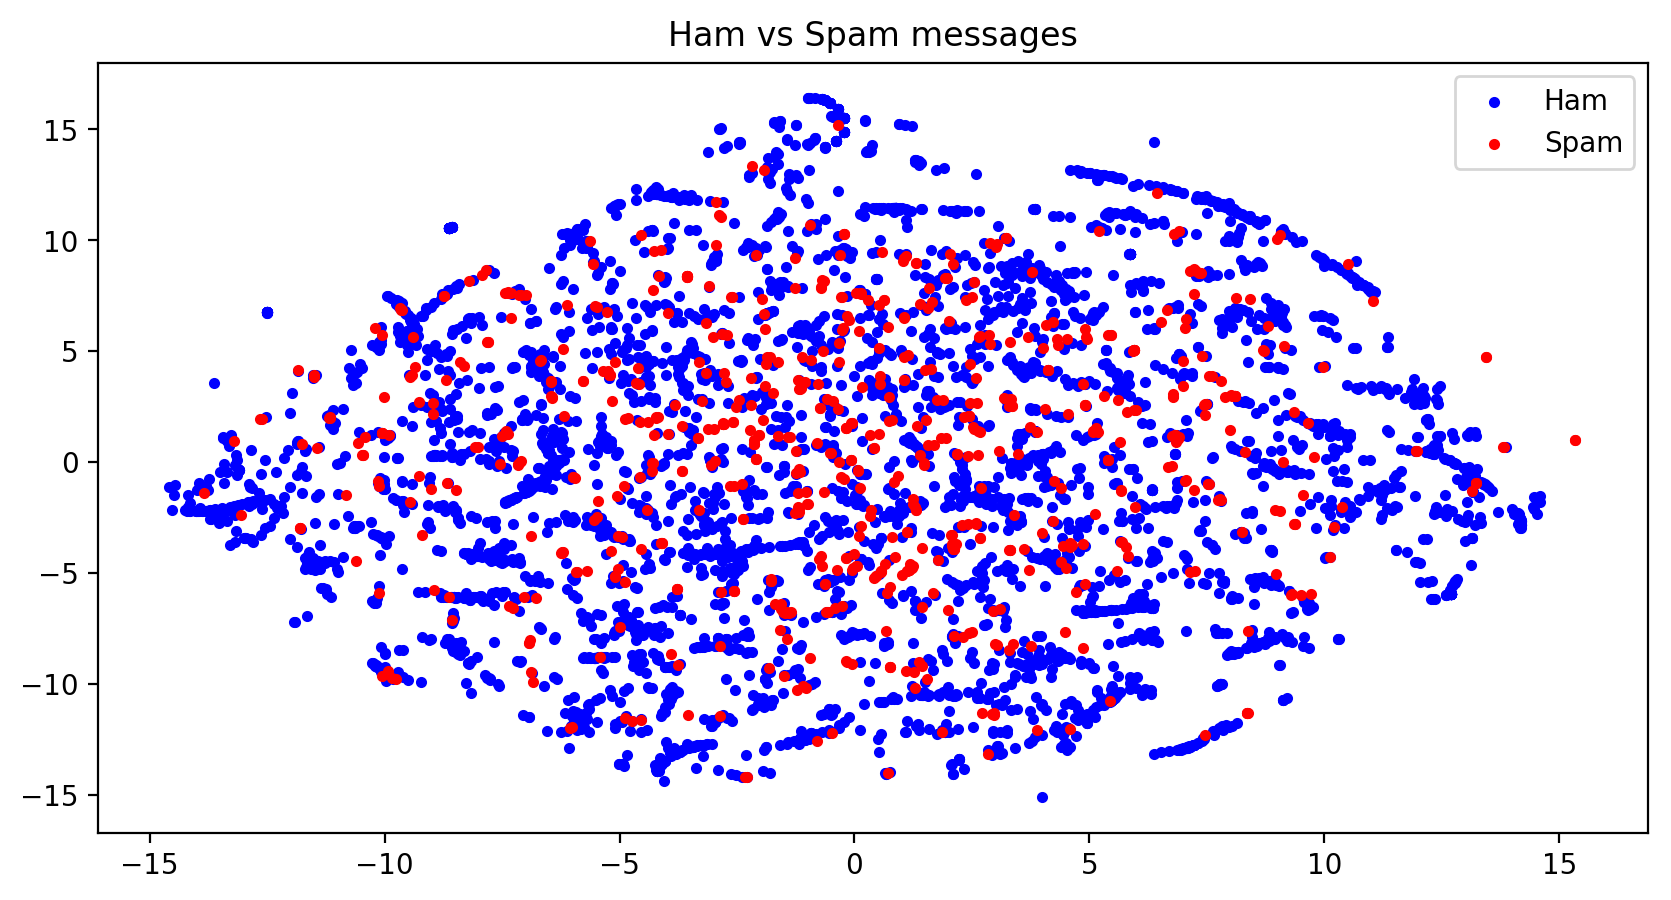
\includegraphics[width = 0.95 \linewidth]{./plot_representations/naive.png}
		\caption{Naive Vector Representation}
		\label{fig: naive}
	\end{subfigure}%
	~ 
	\begin{subfigure}[t]{0.5\textwidth}
		\centering
		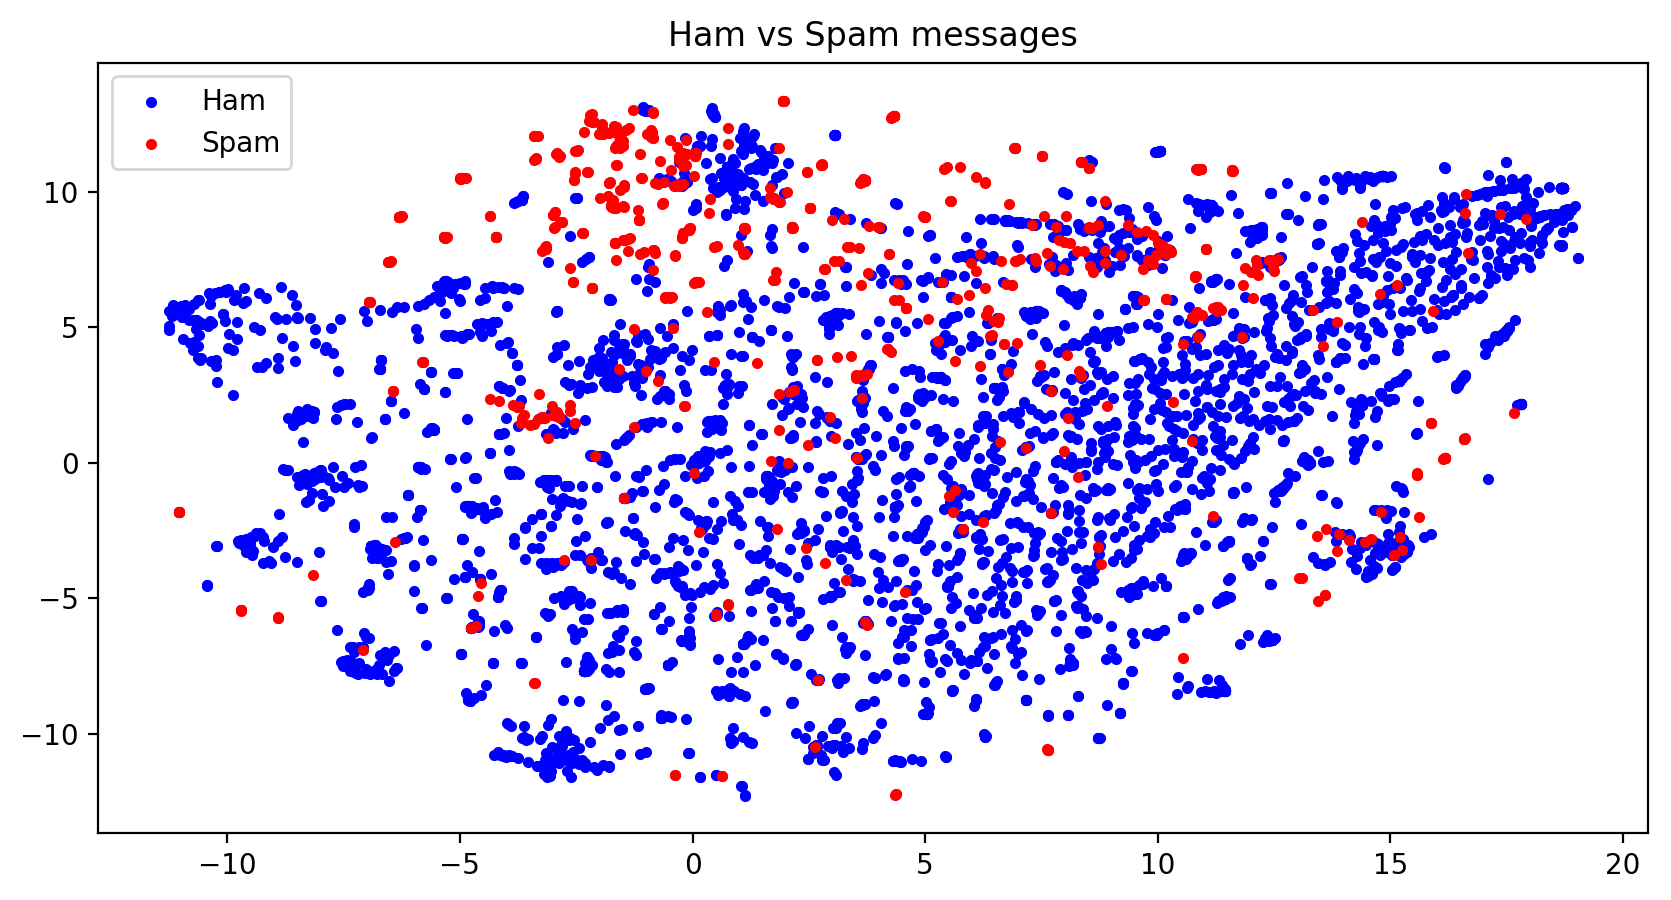
\includegraphics[width = 0.95 \linewidth]{./plot_representations/bow.png}
		\caption{Bag of Words}
		\label{fig: bow}
	\end{subfigure}
	~
	\begin{subfigure}[t]{0.5\textwidth}
		\centering
		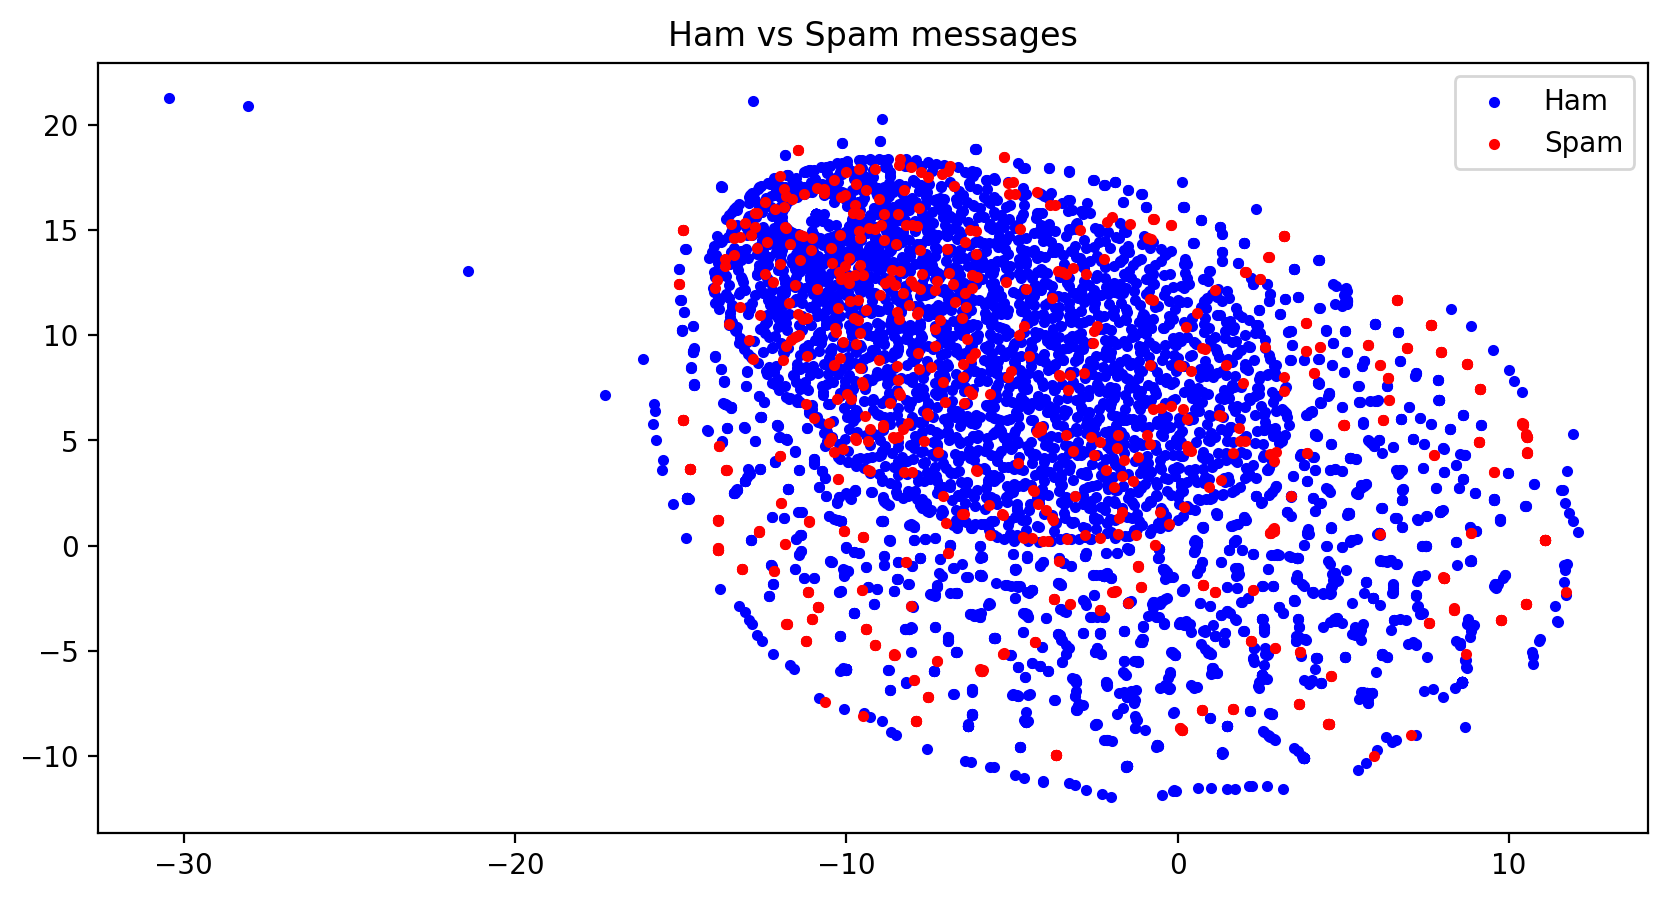
\includegraphics[width = 0.95 \linewidth]{./plot_representations/tfidf.png}
		\caption{Bag of Words with TF-IDF}
		\label{fig: tfidf}
	\end{subfigure}%
	~ 
	\begin{subfigure}[t]{0.5\textwidth}
		\centering
		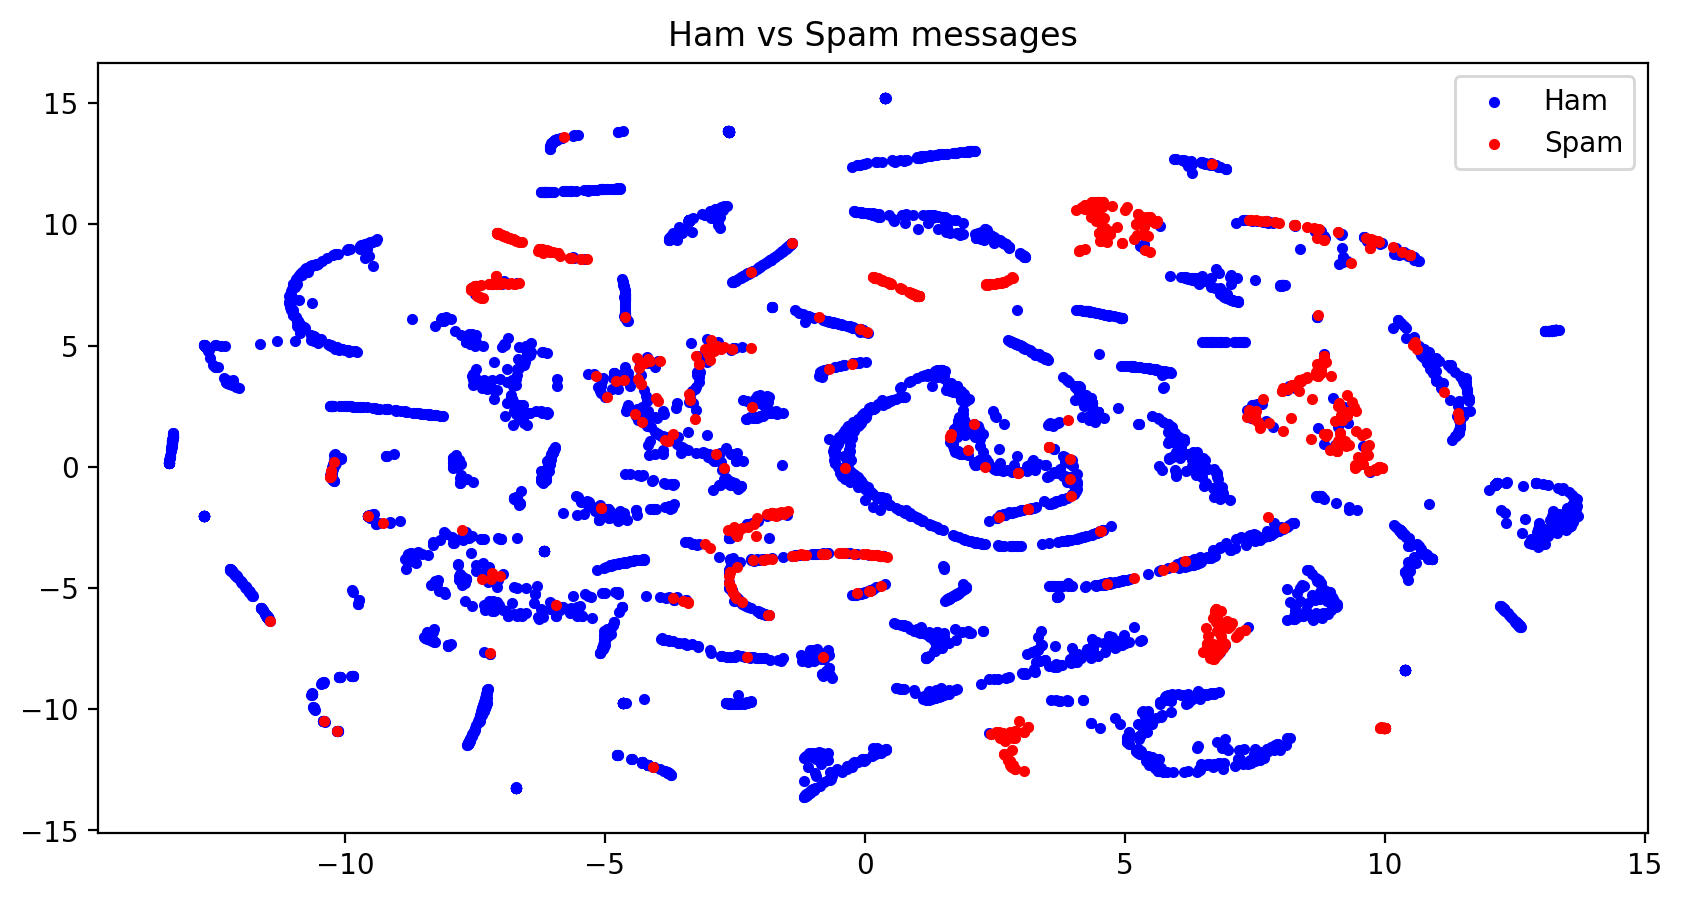
\includegraphics[width = 0.95 \linewidth]{./plot_representations/topics.png}
		\caption{Topic Models}
		\label{fig: topics}
	\end{subfigure}
	~
	\begin{subfigure}[t]{0.5\textwidth}
		\centering
		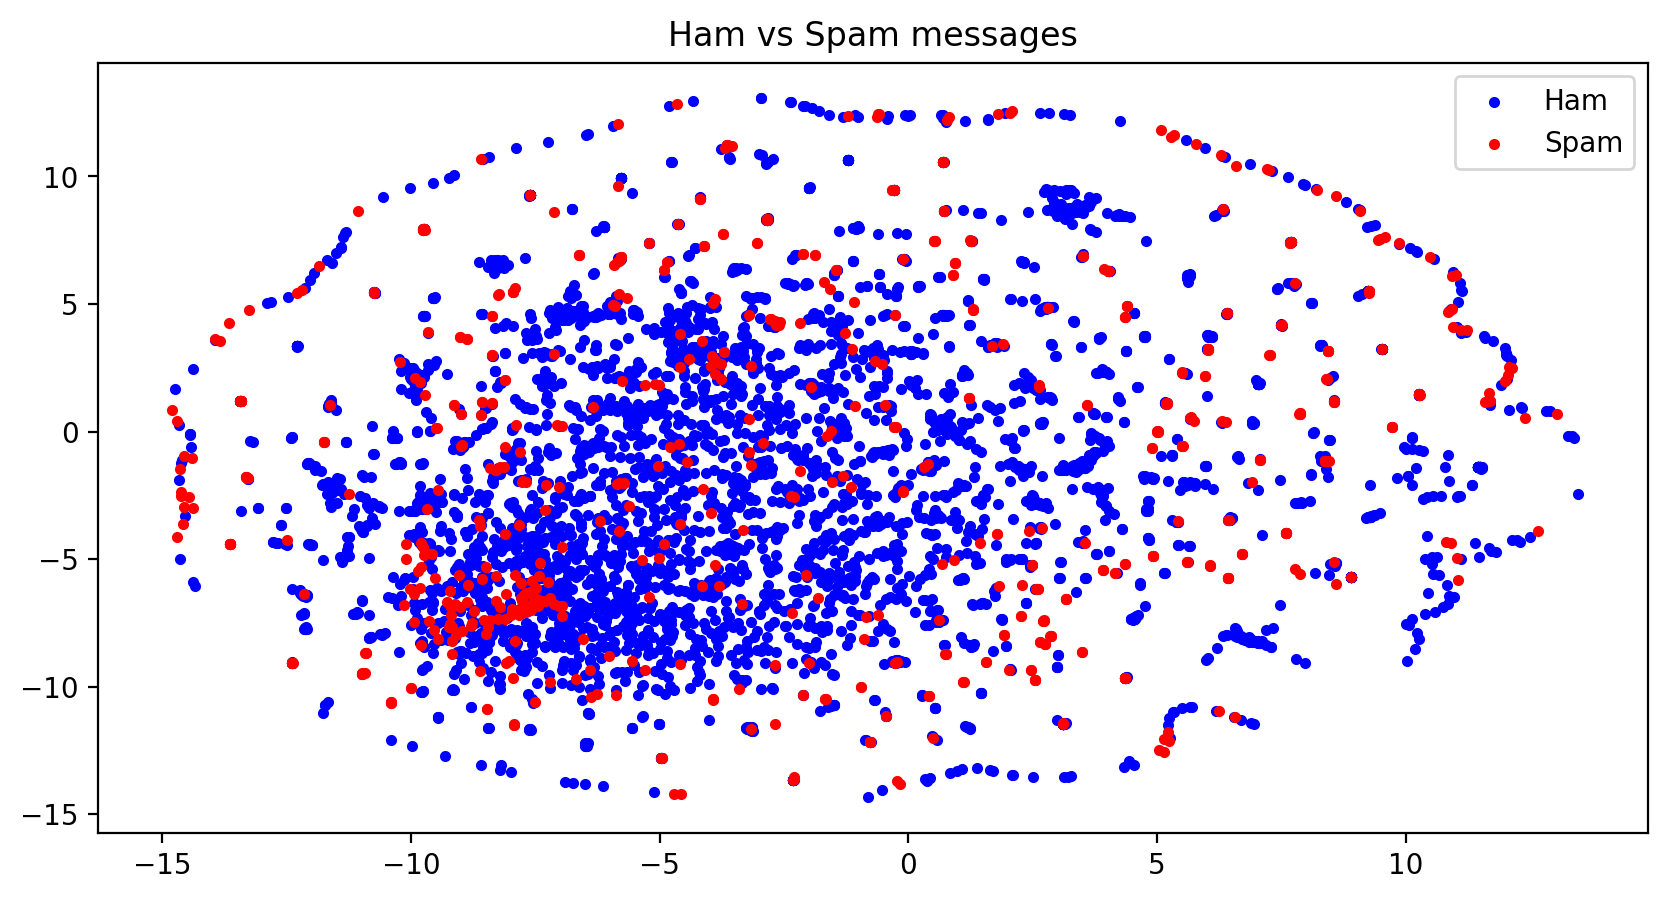
\includegraphics[width = 0.95 \linewidth]{./plot_representations/word_emb.png}
		\caption{Word Embeddings}
		\label{fig: word_emb}
	\end{subfigure}%
	~ 
	\begin{subfigure}[t]{0.5\textwidth}
		\centering
		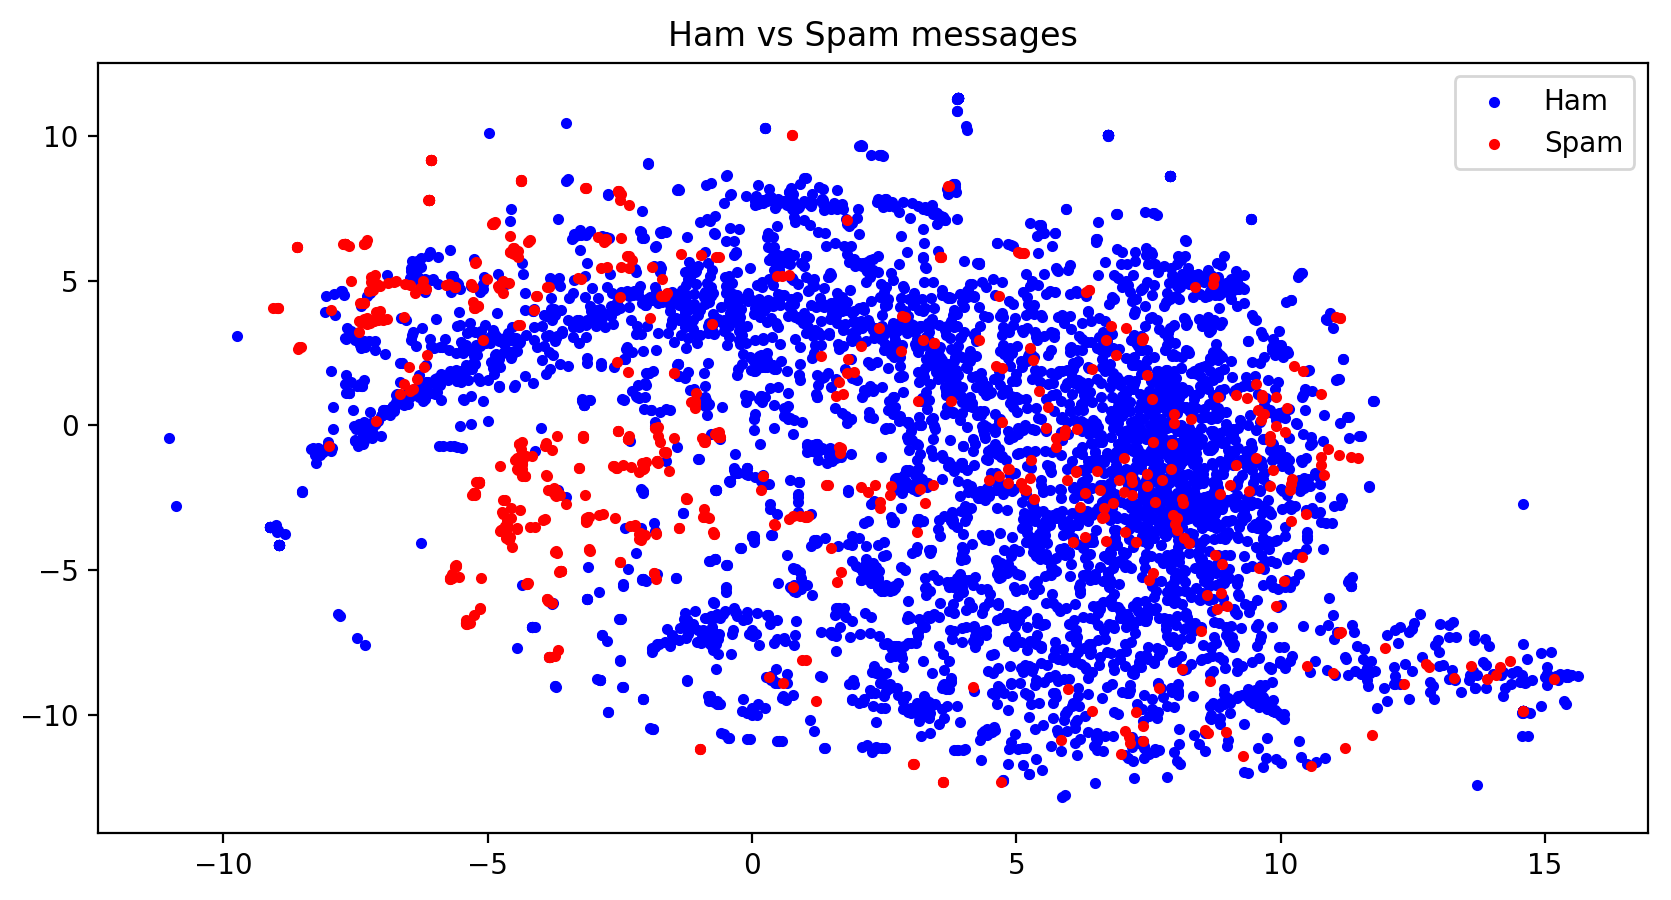
\includegraphics[width = 0.95 \linewidth]{./plot_representations/sent_emb.png}
		\caption{Sentence Embeddings}
		\label{fig: sent_emb}
	\end{subfigure}
	~
	\begin{subfigure}[t]{0.5\textwidth}
		\centering
		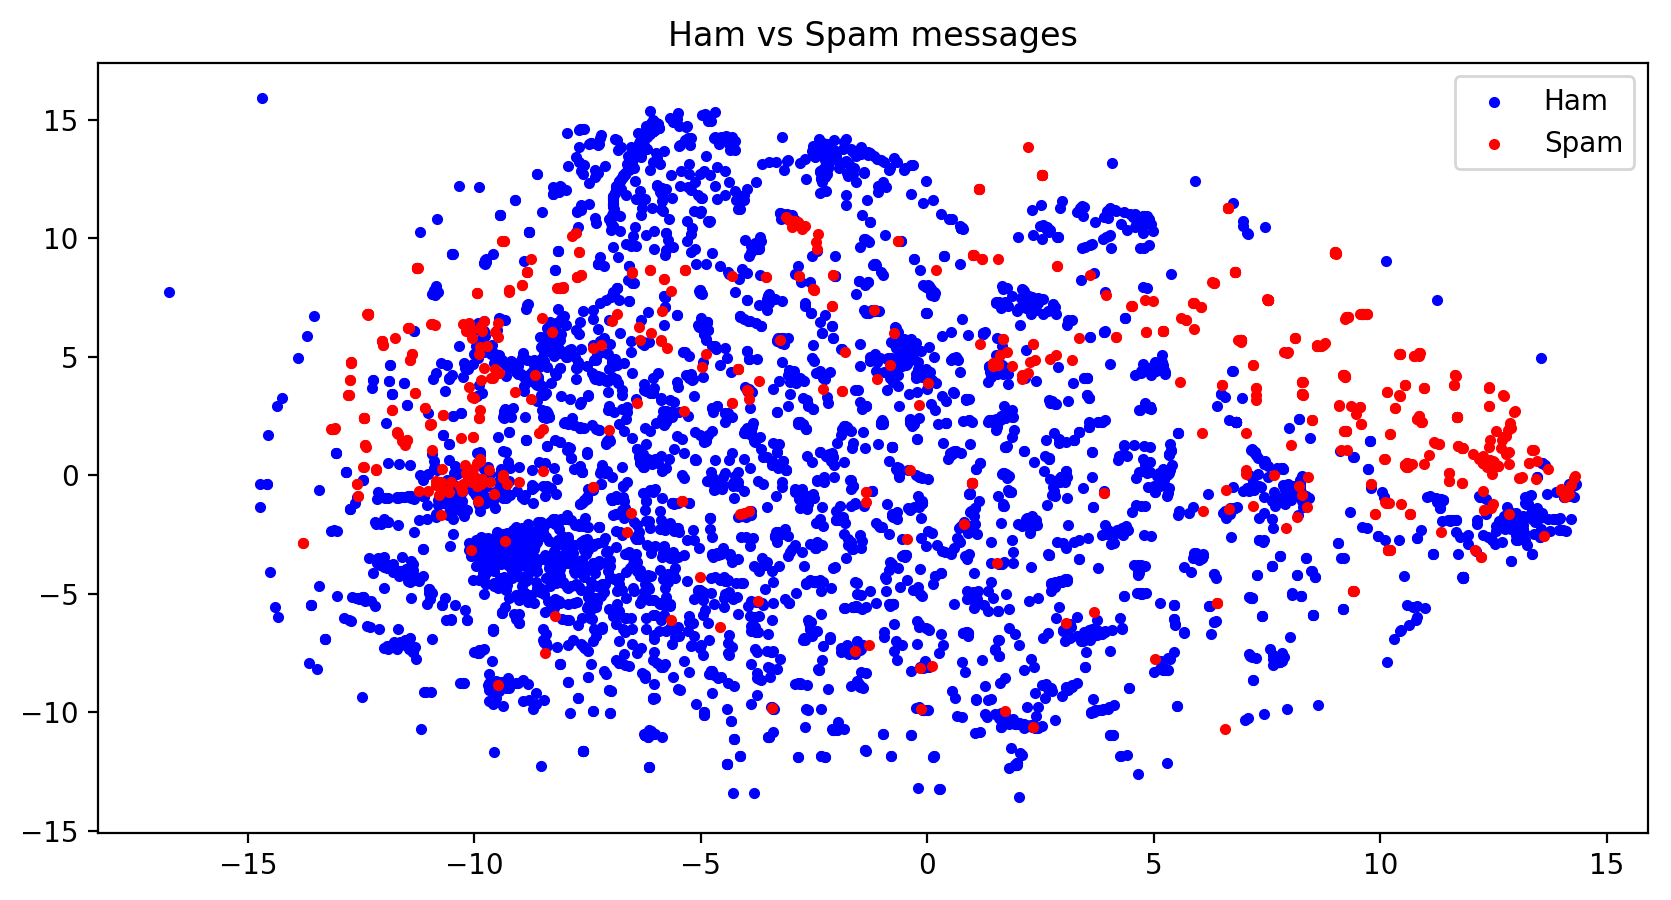
\includegraphics[width = 0.95 \linewidth]{./plot_representations/bow-topics.png}
		\caption{Bag of Words \& Topic Models}
		\label{fig: bow-topics}
	\end{subfigure}
	\caption{2-D visualization using t-SNE of the SMS Spam Collection dataset for each of the message representation models of Section \ref{Representation}.}
	\label{fig: plot_representations}
\end{figure*}

\begin{figure*}[p]
	\centering
	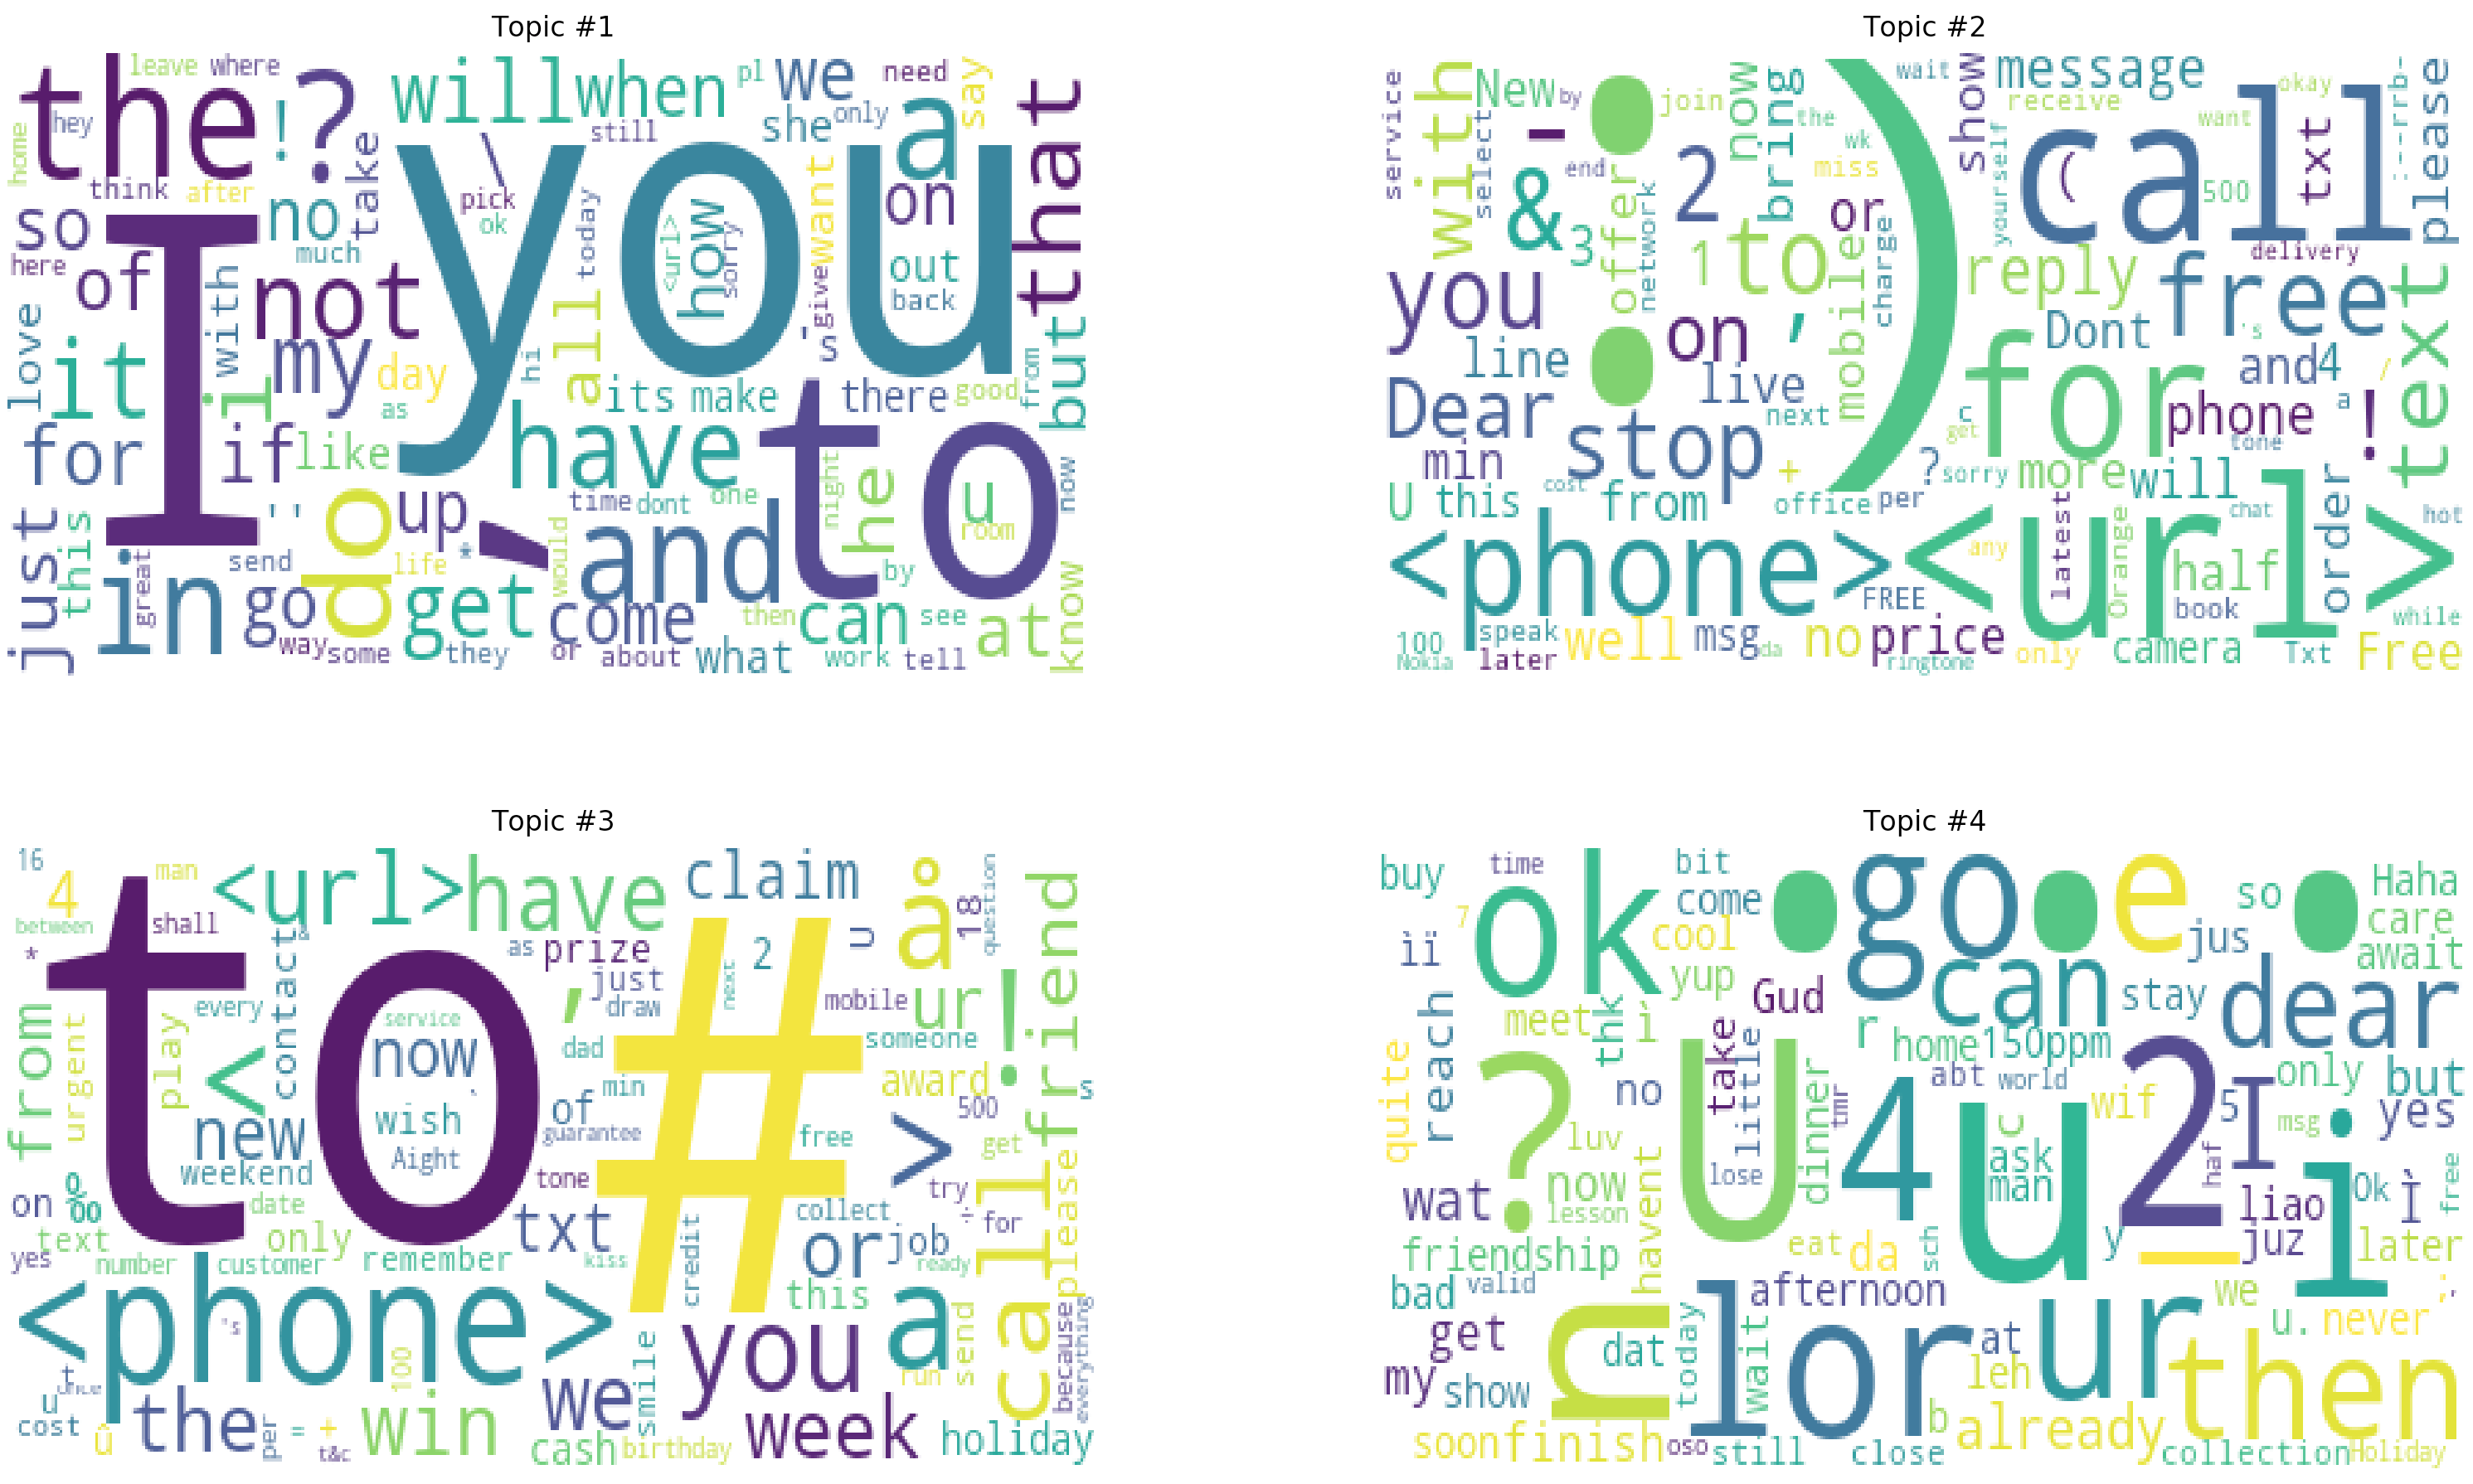
\includegraphics[width = 0.95 \linewidth]{./topics_visualization/word_cloud.png}
	\caption{Word cloud indicating the frequency of each word in a 4-topic message representation model.}
	\label{fig: word_cloud}
\end{figure*}

\begin{landscape}
	\begin{table}[t!]
		\centering
		\caption{Overview of the F1-score achieved by each combination of the employed classification / message representation model.}
		\label{tb: macro_f1}
		\begin{tabular}{@{}rccccccc@{}}
			\toprule
			                                               & Naive & BoW & BoW / TF-IDF & Word Embeddings & Sentence Embeddings & Topics & BoW \& Topics \\ \midrule
			\multicolumn{1}{r|}{Naive Bayes (Bernoulli)}   & 0.707 &     & 0.951        &                 & 0.669               & 0.460  & 0.951         \\
			\multicolumn{1}{r|}{Naive Bayes (Multinomial)} & 0.682 &     & 0.962        &                 &                     & 0.460  & \textbf{0.971}\\
			\multicolumn{1}{r|}{Naive Bayes (Gaussian)}    & 0.159 &     & 0.748        &                 & 0.573               & 0.837  & 0.748         \\
			\multicolumn{1}{r|}{Logistic Regression}       & 0.600 &     & 0.966        &                 & 0.912               & 0.880  & 0.964         \\
			\multicolumn{1}{r|}{Decision Tree}             & 0.799 &     & 0.960        &                 & 0.793               & 0.888  & 0.950         \\
			\multicolumn{1}{r|}{Random Forest}             & 0.826 &     & 0.964        &                 & 0.834               & 0.895  & 0.956         \\
			\multicolumn{1}{r|}{SVM (Linear)}              &       &     & 0.968        &                 & 0.918               & 0.878  & 0.962         \\
			\multicolumn{1}{r|}{SVM (RBF)}                 & 0.691 &     & 0.460        &                 & 0.805               & 0.876  & 0.460         \\
			\multicolumn{1}{r|}{AdaBoost}                  & 0.836 &     & 0.959        &                 & 0.905               & 0.878  & 0.951         \\
			\multicolumn{1}{r|}{Feed-forward Neural Net}   & 0.659 &     & 0.951        &                 & 0.931               & 0.460  & 0.956         \\
			\multicolumn{1}{r|}{Recurrent Neural Net}      &       &     &              & \textbf{0.978}  &                     &        &               \\
			\multicolumn{1}{r|}{Convolutional Neural Net}  &       &     &              & \textbf{0.976}  &                     &        &               \\ \bottomrule
		\end{tabular}
	\end{table}
\end{landscape}

\begin{landscape}
	\begin{table}[t!]
		\centering
		\caption{Overview of the training and testing time required by each combination of the employed classification / message representation model.}
		\label{tb: time}
		\begin{tabular}{@{}r|lclclclclclclc@{}}
			\toprule
			                          & \multicolumn{2}{c}{Naive}         & \multicolumn{2}{c}{BoW}           & \multicolumn{2}{c}{BoW / TF-IDF}  & \multicolumn{2}{c}{Word Embeddings} & \multicolumn{2}{c}{Sentence Embeddings} & \multicolumn{2}{c}{Topics}             & \multicolumn{2}{c}{BoW \& Topics}            \\
			\multicolumn{1}{l|}{}     & \multicolumn{1}{c}{Train} & Test  & \multicolumn{1}{c}{Train} & Test  & \multicolumn{1}{c}{Train} & Test  & \multicolumn{1}{c}{Train} & Test    & \multicolumn{1}{c}{Train}     & Test    & \multicolumn{1}{c}{Train}    & Test    & \multicolumn{1}{c}{Train}    & Test          \\ \midrule
			Naive Bayes (Bernoulli)   & 0.011                     & 0.001 & 0.373                     & 0.092 & 0.353                     & 0.086 &                           &         & 0.059                         & 0.013   & 0.001                        & 0.000   & 0.607                        & 0.144         \\
			Naive Bayes (Multinomial) & 0.004                     & 0.000 & 0.172                     & 0.033 & 0.164                     & 0.032 &                           &         &                               &         & 0.001                        & 8.249   & \textbf{0.229}               & \textbf{0.052}\\
			Naive Bayes (Gaussian)    & 0.011                     & 0.002 & 0.468                     & 0.118 & 0.500                     & 0.126 &                           &         & 0.038                         & 0.008   & 0.001                        & 0.000   & 0.654                        & 0.181         \\
			Logistic Regression       & 0.097                     & 0.000 & 0.925                     & 0.024 & 0.901                     & 0.032 &                           &         & 0.200                         & 0.001   & 0.021                        & 0.000   & 0.963                        & 0.050         \\
			Decision Tree             & 0.041                     & 0.000 & 9.982                     & 0.030 & 6.426                     & 0.026 &                           &         & 1.936                         & 0.001   & 0.013                        & 0.000   & 12.060                       & 0.045         \\
			Random Forest             & 0.085                     & 0.007 & 4.190                     & 0.136 & 2.616                     & 0.087 &                           &         & 0.902                         & 0.008   & 0.107                        & 0.006   & 4.380                        & 0.188         \\
			SVM (Linear)              &                           &       & 17.196                    & 3.791 & 28.913                    & 7.335 &                           &         & 2.415                         & 0.356   & 0.035                        & 0.005   & 15.208                       & 3.148         \\
			SVM (RBF)                 & 3.513                     & 0.834 & 45.042                    & 11.604& 40.929                    & 9.913 &                           &         & 3.866                         & 0.780   & 0.099                        & 0.016   & 41.349                       & 10.146        \\
			AdaBoost                  & 0.411                     & 0.013 & 17.084                    & 0.205 & 23.387                    & 0.216 &                           &         & 14.000                        & 0.024   & 0.169                        & 0.009   & 23.845                       & 0.219         \\
			Feed-forward Neural Net   & 0.179                     & 0.002 & 4.149                     & 0.049 & 13.387                    & 0.062 &                           &         & 1.565                         & 0.011   & 0.058                        & 0.001   & 6.795                        & 0.050         \\
			Recurrent Neural Net      &                           &       &                           &       &                           &       & 11.210                    & 0.093   &                               &         &                              &         &                              &               \\
			Convolutional Neural Net  &                           &       &                           &       &                           &       & 21.489                    & 0.225   &                               &         &                              &         &                              &               \\ \bottomrule
		\end{tabular}
	\end{table}
\end{landscape}

\clearpage

% \bibliographystyle{IEEEtran}
% \bibliographystyle{plainnat}
\bibliography{bibliography}
\bibliographystyle{aaai}

\end{document}
